\section{User Interface and Orchestration}
\subsection{State}
\subsubsection{Design}
A single window approach worked well initially, however, as requirements grew and additional features and requirements resulted in more views, state management required a complete design. Every UI element existed in the same \texttt{MainWindow.xaml} file due to the complexity of creating new interfaces and transitioning between them. To manage this, I designed a state machine as a private struct owned by the \texttt{MainWindow} class to handle the transitions between the different states of the application. Here is a diagram to demonstrate

\begin{figure}[H]
    \centering
    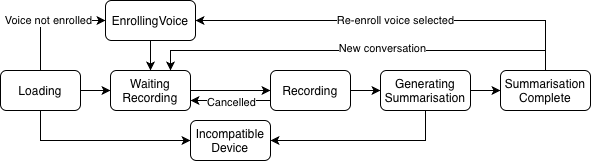
\includegraphics[width=1\linewidth]{chapters/design_implementation/state.drawio-2.png}
    \caption{A state diagram with transitions labelled if unclear}
    \label{fig:state}
\end{figure}

\subsubsection{Implementation}
In practice, \texttt{enum class AppState{};} in the \texttt{MainWindow} class holds each state value with a setter function \texttt{void SetAppState(AppState state);} to change state. This function handles all states of all UI components, modifying the visibility and activity depending on which state the application is in. This approach gives a single UI application the flexibility to display the correct components depending on the stage of the application

\subsection{UI Design/Implementation}
The user interface took several iterations, with feedback from my internal and external supervisors, along with 2 NHS clients, resulting in a pastel background with bold button colours to guide the user through the standard workflow of the application.

The background colours represent this project's participants. The blue in the bottom left represents the NHS's logo fading into a purple representing UCL before finishing with a yellow, my favourite colour. This also provides an appeasing user interface aesthetic while matching the typical colours found in AI powered applications. All buttons are rounded to match the Windows 11 style.

\begin{figure}[H]
    \centering
    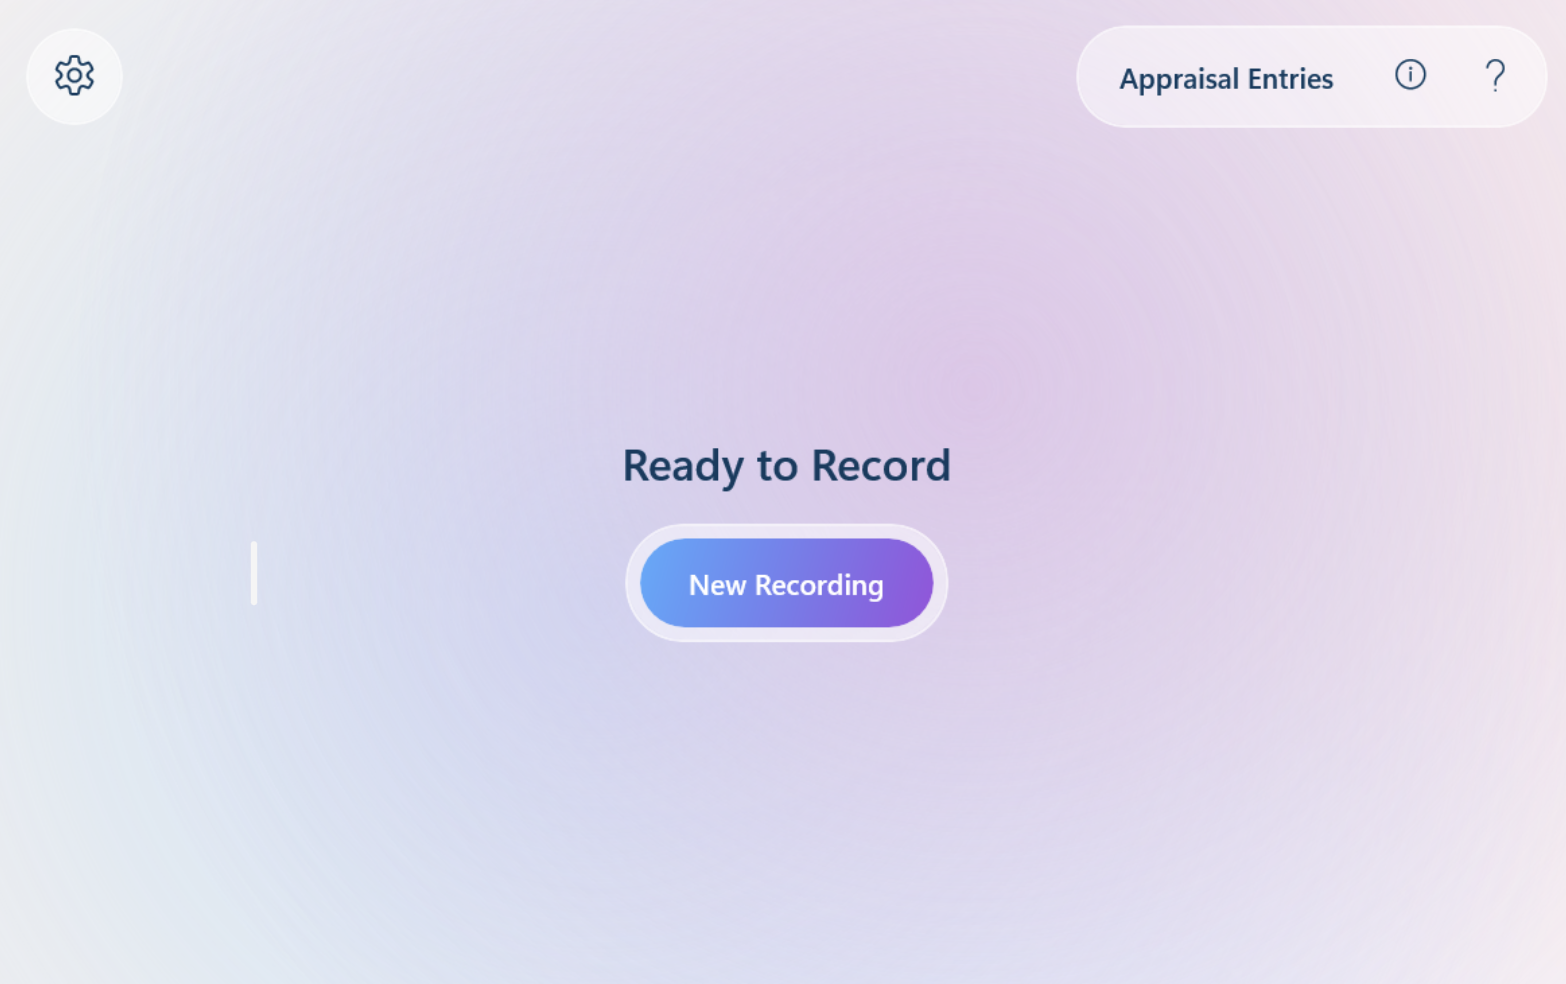
\includegraphics[width=0.48\linewidth]{ui1.png}\hfill
    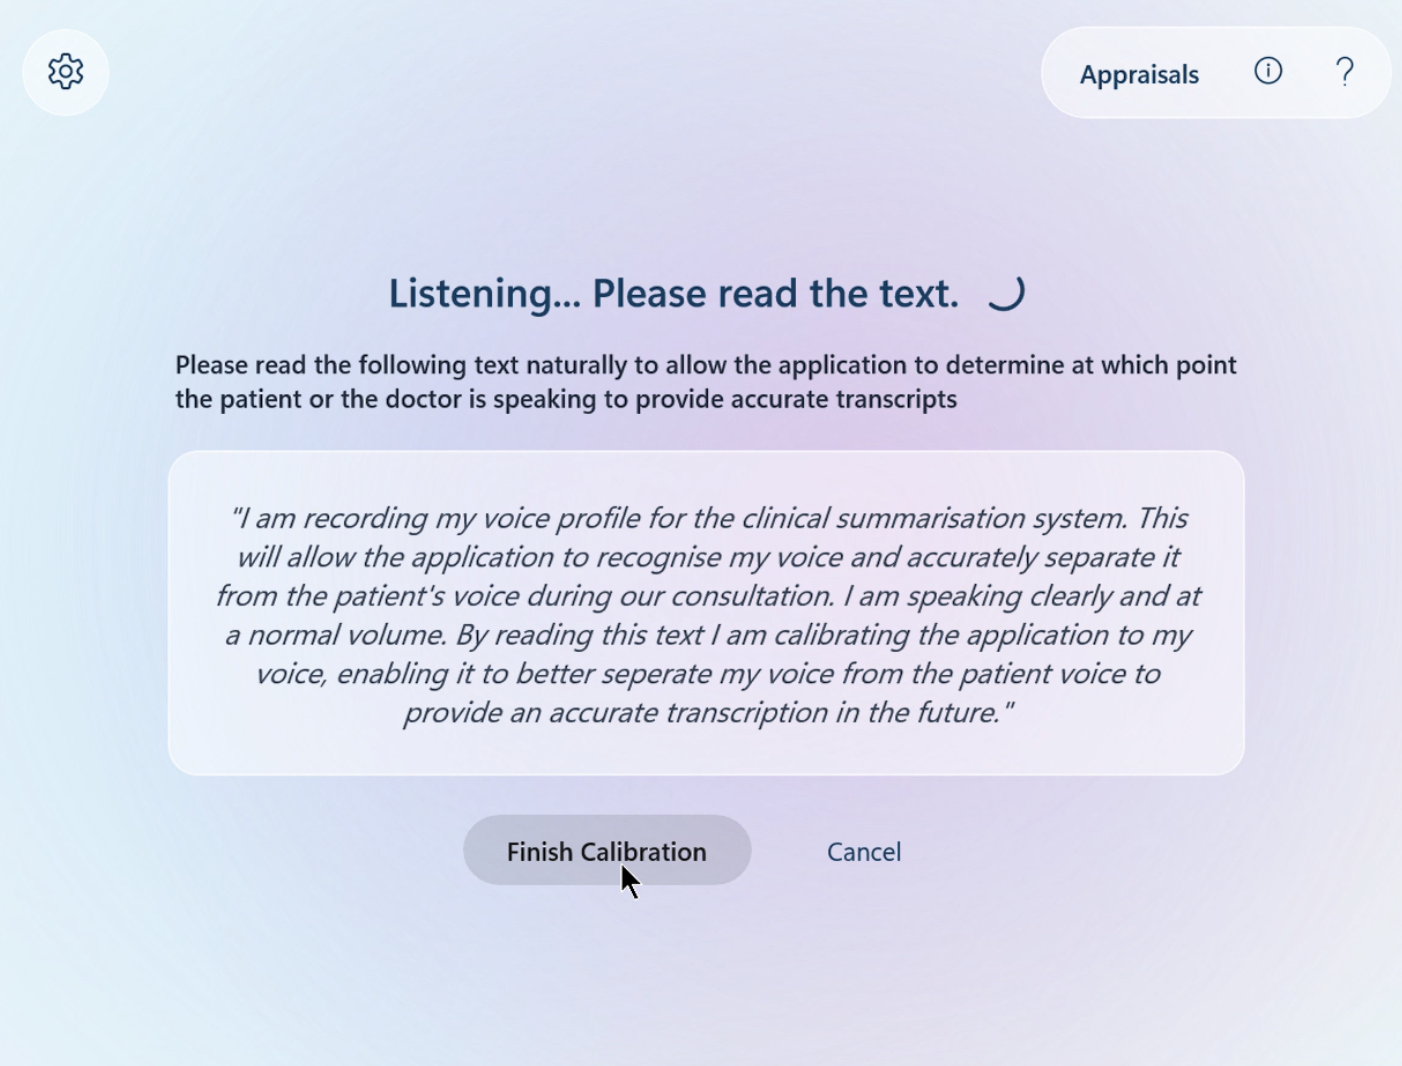
\includegraphics[width=0.48\linewidth]{ui2.png}
    
    \vspace{1em} % Adds a little vertical space between the rows
    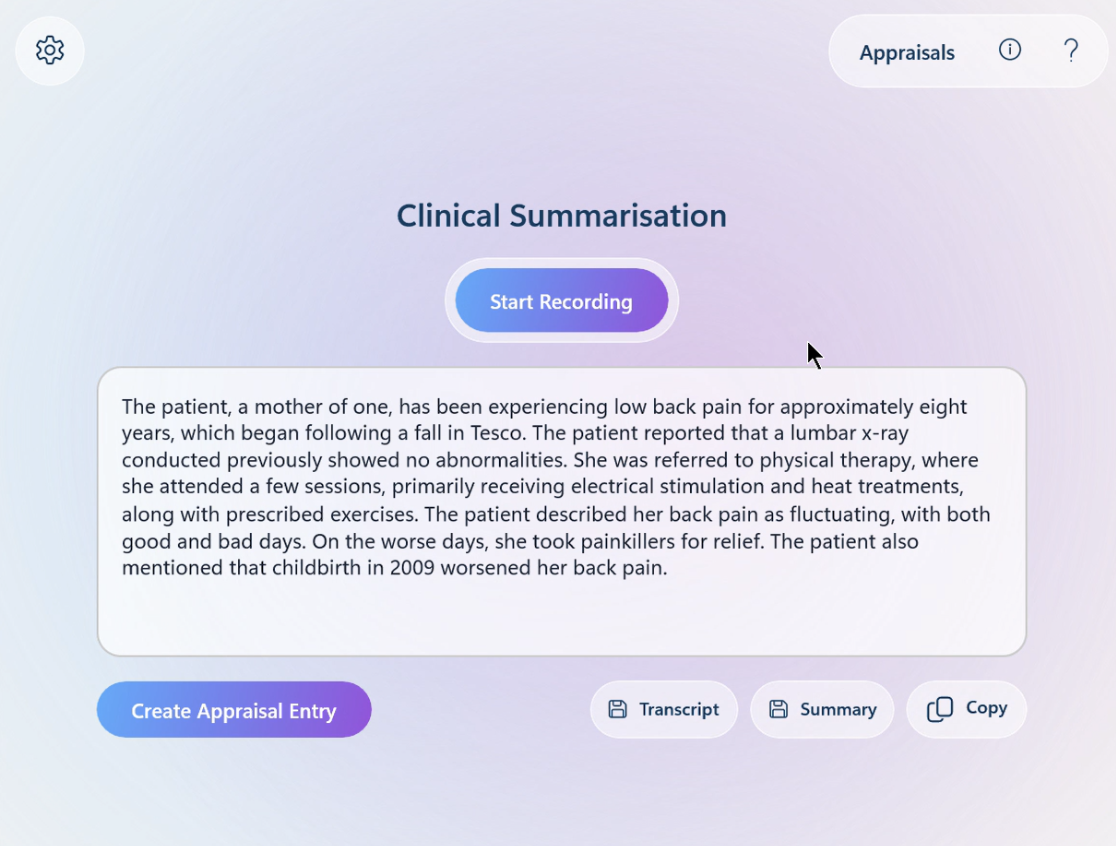
\includegraphics[width=0.48\linewidth]{ui3.png}\hfill
    
\includegraphics[width=0.48\linewidth]{ui4.png}
    
    \caption{Top left: WaitingRecording state, top right: EnrollingVoice state, bottom left: SummarisationComplete state, bottom right: Recording state}
    \label{fig:UI_grid}
\end{figure}

Loading, IncompatibleDevice and GeneratingSummarisation states all have the same UI as WaitingRecording with no "Start Recording" button. 

The persistent settings, information and help bar at the top of the application persists over all views and states for ease of access. These flyout menus expand to the following:
\begin{figure}[H]
    \centering
    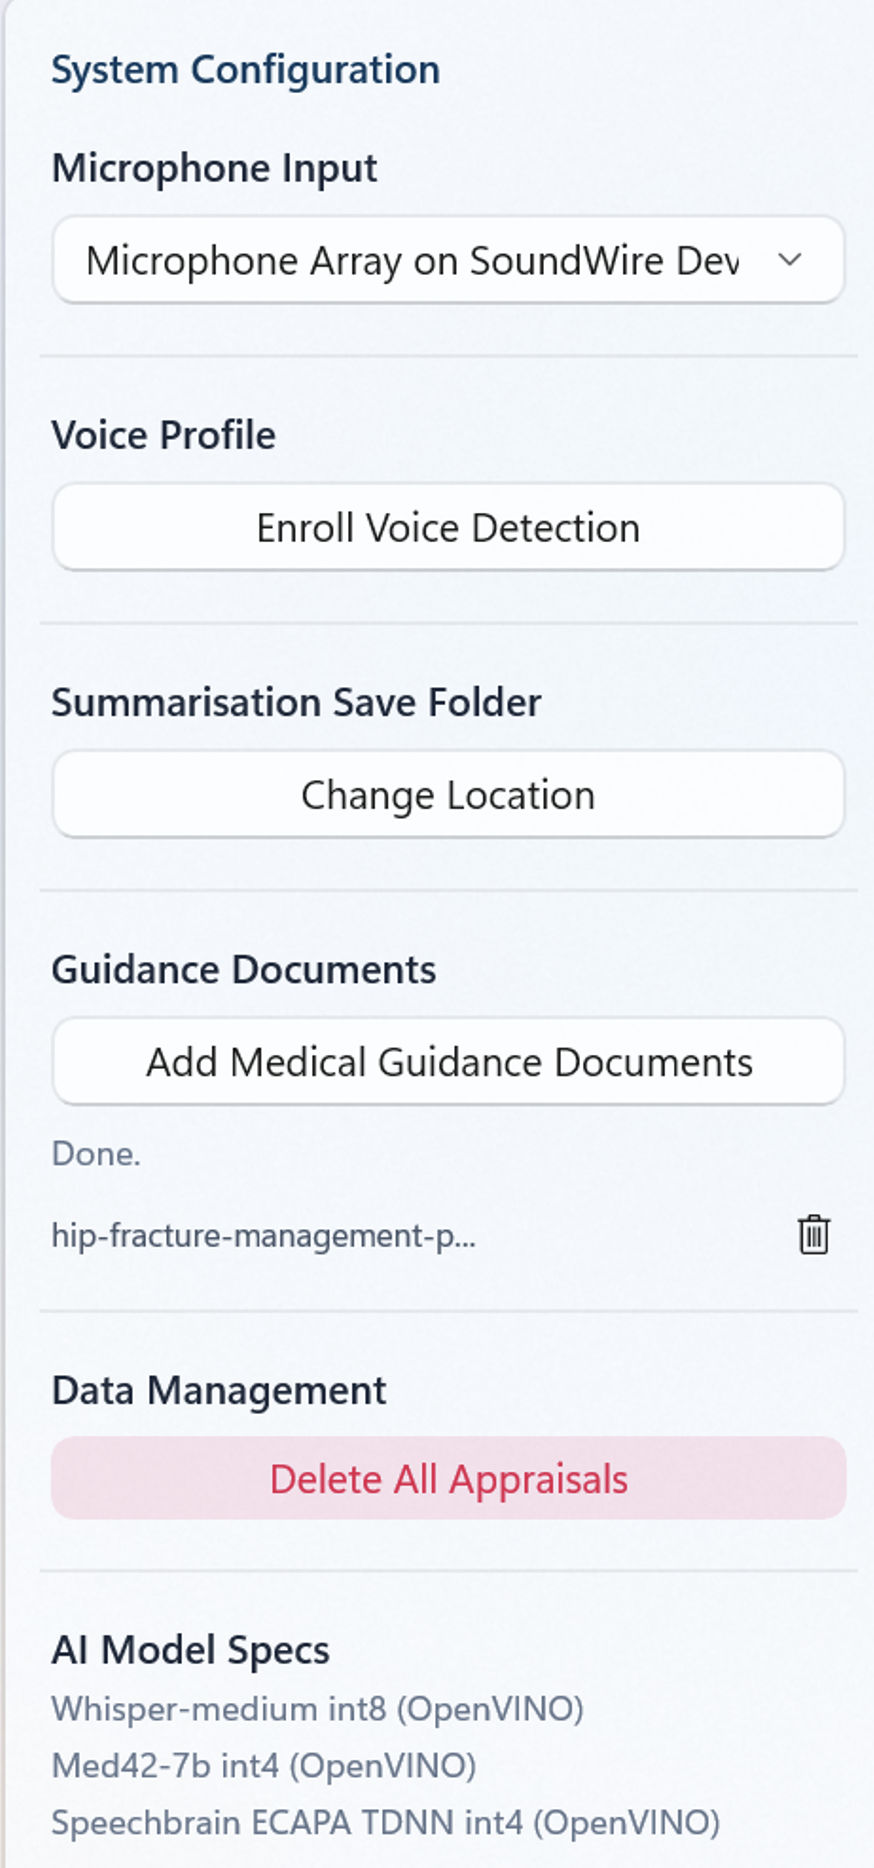
\includegraphics[width=0.32\linewidth]{ui5.png}\hfill
    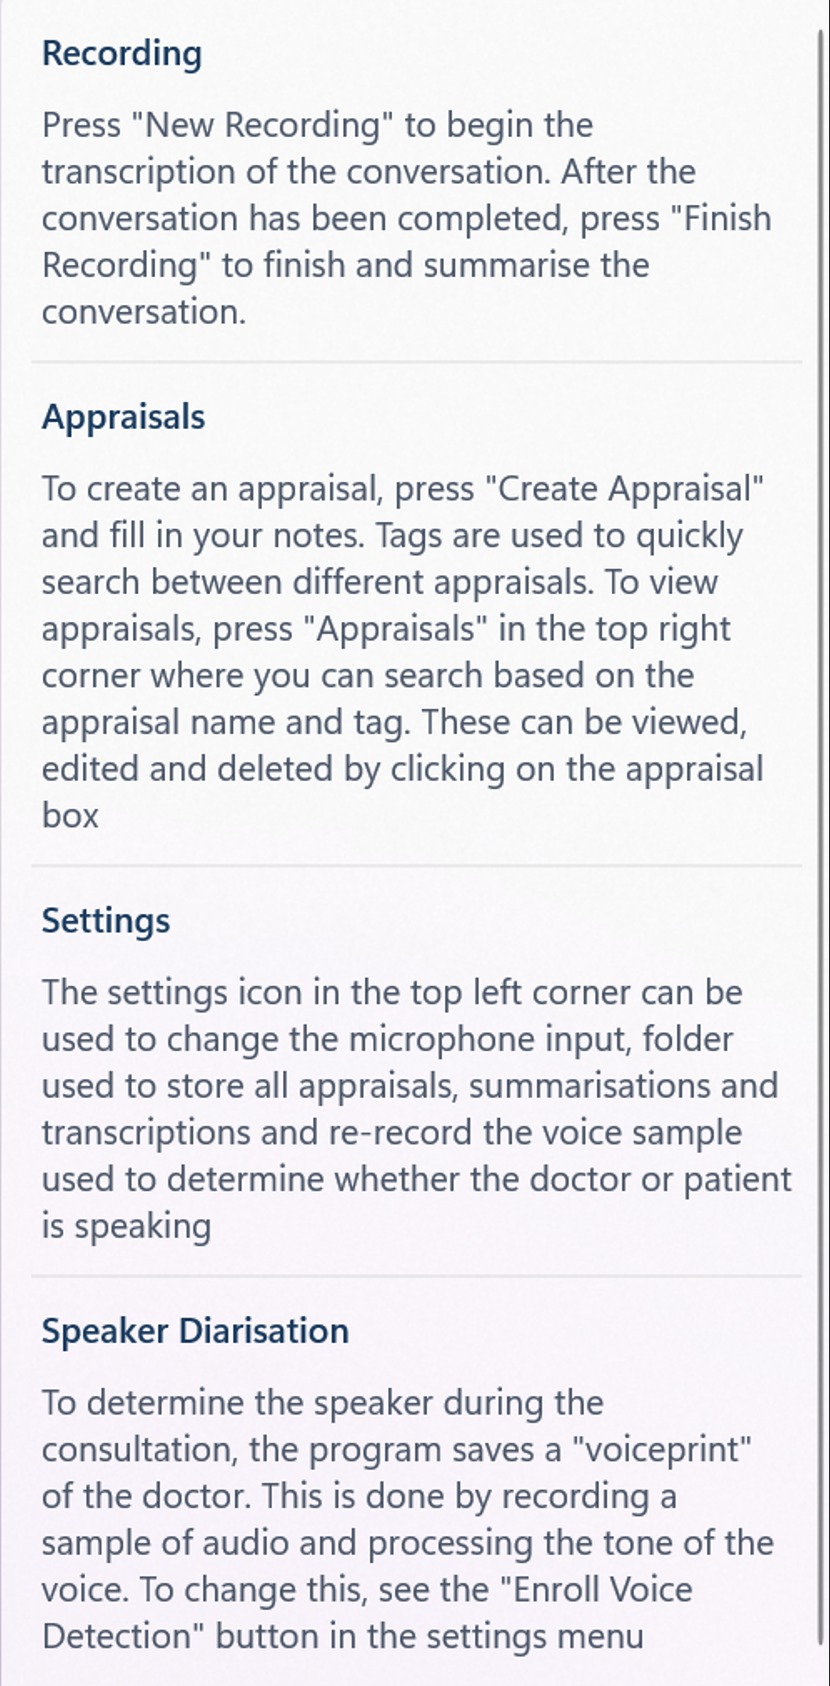
\includegraphics[width=0.32\linewidth]{ui6.png}\hfill
    
\includegraphics[width=0.32\linewidth]{ui7.png}
    
    \caption{Left: Settings flyout, Middle: Help flyout, Right: Information flyout}
    \label{fig:UI_grid_flyouts}
\end{figure}

As shown in the settings flyout, the doctor can re-record their voice embedding, choose their microphone input and change the default save location. Deleting appraisals and managing guidance documents will be covered (TODO reference)

\subsection{Windows Filesystem Interactions}
\subsubsection{Design}
To provide flexibility to the user, the Clinical Summarisation screen contains buttons enabling the saving of the transcription and summarisation, and copying the summarisation to the user's clipboard. This uses the WinRT API to open the file explorer to the path determined by the default save folder in the settings. Next, the filename prefix \texttt{<YYYY-DD-MM>\_<Appraisal/Transcription/Summary>\_} is added to ensure the NHS file saving format is retained.

\subsubsection{Implementation}
The implementation required additional complexity due to the WinRT API not supporting the file explorer opening at a pre-determined path. Therefore, this implementation used the older \texttt{Microsoft::WRL::ComPtr<ISaveFile>} interface for file access. The WinRT implementation was simple:
\begin{verbatim}
    // some code has been omitted for brevity
    winrt::Windows::Storage::Pickers::FileSavePicker savePicker;
    winrt::Windows::Storage::StorageFile file = co_await
                                savePicker.PickSaveFileAsync();
\end{verbatim}  

Compared to the verbose ISaveFile interface implementation
\begin{verbatim}
    // some code has been omitted for brevity
    ::Microsoft::WRL::ComPtr<IFileSaveDialog> dialog;
    winrt::check_hresult(CoCreateInstance(
        CLSID_FileSaveDialog, nullptr, CLSCTX_ALL, IID_PPV_ARGS(&dialog))
    );
    ::Microsoft::WRL::ComPtr<IShellItem> folderItem;
    if (SUCCEEDED(SHCreateItemFromParsingName(savedFolder.Path().c_str(),       
                                    nullptr, IID_PPV_ARGS(&folderItem)))) {
        dialog->SetFolder(folderItem.Get());
    }
\end{verbatim}



